\section{Overview}

This chapter presents our methodology for integrating Deep Descriptive Clustering (DDC) principles into the Deep Embedded Clustering with Consensus Representations (DECCS) framework. Our approach addresses the dual objectives of achieving high-precision clustering while maintaining interpretability through semantic supervision.

\subsection{Methodological Contributions}

Our methodology makes three key contributions:

\begin{enumerate}
    \item \textbf{Semantic-Guided Representation Learning}: We extend traditional autoencoder architectures with a tag prediction branch that enforces semantic consistency in the learned embedding space.

    \item \textbf{Consensus Clustering with Semantic Grounding}: We adapt DECCS's ensemble clustering approach to operate on semantically-supervised embeddings, creating consensus representations that are both robust and interpretable.

    \item \textbf{Attribute-Based Cluster Explanation}: We develop a post-hoc explanation mechanism that characterizes clusters using human-interpretable semantic attributes.
\end{enumerate}

\subsection{Research Design}

Our research follows a comparative experimental design with four modes:

\begin{description}
    \item[\textbf{AE (Baseline)}:] Pure reconstruction-based autoencoder without semantic supervision, establishing performance lower bound.

    \item[\textbf{Oracle}:] Concatenation of learned embeddings with ground-truth symbolic tags, establishing performance upper bound.

    \item[\textbf{CAE (Constrained Autoencoder)}:] Autoencoder with tag prediction supervision, our primary contribution for interpretable clustering.

    \item[\textbf{DECCS}:] Full integration with consensus clustering mechanism and semantic supervision (designed but partially implemented).
\end{description}

Figure~\ref{fig:methodology_overview} illustrates the overall pipeline.

\begin{figure}[H]
    \centering
    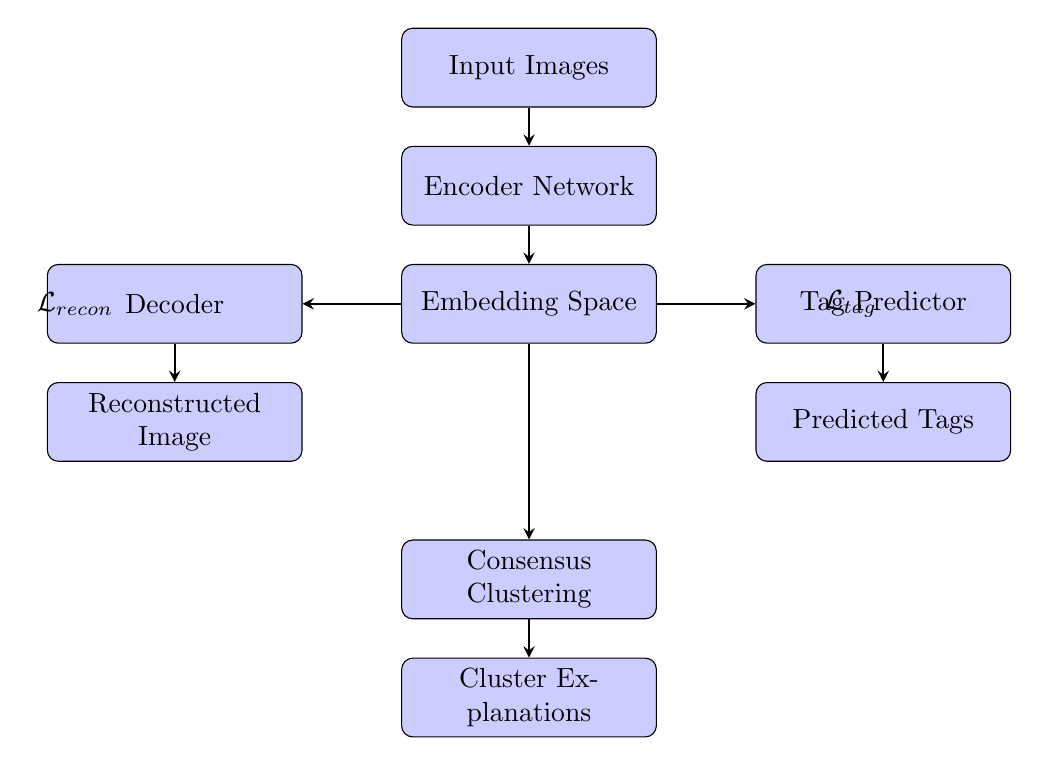
\begin{tikzpicture}[
        node distance=1.5cm,
        block/.style={rectangle, draw, fill=blue!20, text width=3cm, text centered, rounded corners, minimum height=1cm},
        arrow/.style={->, >=stealth, thick}
    ]

        \node (input) [block] {Input Images};
        \node (encoder) [block, below of=input] {Encoder Network};
        \node (embedding) [block, below of=encoder] {Embedding Space};
        \node (decoder) [block, left of=embedding, xshift=-3cm] {Decoder};
        \node (tagpred) [block, right of=embedding, xshift=3cm] {Tag Predictor};
        \node (recon) [block, below of=decoder] {Reconstructed Image};
        \node (tags) [block, below of=tagpred] {Predicted Tags};
        \node (consensus) [block, below of=embedding, yshift=-2cm] {Consensus Clustering};
        \node (explanation) [block, below of=consensus] {Cluster Explanations};

        \draw[arrow] (input) -- (encoder);
        \draw[arrow] (encoder) -- (embedding);
        \draw[arrow] (embedding) -- (decoder);
        \draw[arrow] (embedding) -- (tagpred);
        \draw[arrow] (decoder) -- (recon);
        \draw[arrow] (tagpred) -- (tags);
        \draw[arrow] (embedding) -- (consensus);
        \draw[arrow] (consensus) -- (explanation);

        \node[draw=none, text width=2.5cm, align=left] at (-5, -3) {$\mathcal{L}_{recon}$};
        \node[draw=none, text width=2.5cm, align=left] at (5, -3) {$\mathcal{L}_{tag}$};

    \end{tikzpicture}
    \caption{Overview of our integrated methodology combining semantic supervision, representation learning, and consensus clustering}
    \label{fig:methodology_overview}
\end{figure}

\section{Dataset Preparation}

\subsection{Animals with Attributes 2 (AwA2) Dataset}

The AwA2 dataset \citep{Xian2019, Lampert2014} is a benchmark for attribute-based recognition, containing:

\begin{itemize}
    \item \textbf{37,322 images} across 50 animal classes
    \item \textbf{85 semantic attributes} per class (e.g., furry, quadrupedal, swims)
    \item \textbf{Continuous attribute values} in range [0, 1], representing attribute strength
    \item \textbf{Class-level annotations}: Each of 50 classes has an 85-dimensional attribute vector
\end{itemize}

\subsection{Semantic Attribute Structure}

The predicate matrix $\mathbf{P} \in \mathbb{R}^{C \times T}$ encodes semantic attributes for $C=50$ classes and $T=85$ attributes. For class $c$, the attribute vector is:

\begin{equation}
    \mathbf{p}_c = [p_{c,1}, p_{c,2}, \ldots, p_{c,85}]^T
\end{equation}

where $p_{c,t} \in [0, 1]$ represents the strength of attribute $t$ for class $c$.

\textbf{Example attributes include:}
\begin{multicols}{3}
    \begin{itemize}
        \item black
        \item white
        \item blue
        \item brown
        \item gray
        \item orange
        \item red
        \item yellow
        \item patches
        \item spots
        \item stripes
        \item furry
        \item hairless
        \item toughskin
        \item big
        \item small
        \item bulbous
        \item lean
        \item flippers
        \item hands
        \item hooves
        \item pads
        \item paws
        \item longleg
        \item longneck
        \item tail
        \item chewteeth
        \item meatteeth
        \item buckteeth
        \item strainteeth
        \item horns
        \item claws
        \item tusks
        \item smelly
        \item flys
        \item hops
        \item swims
        \item tunnels
        \item walks
        \item fast
        \item slow
        \item strong
        \item weak
        \item muscle
        \item bipedal
        \item quadrapedal
        \item active
        \item inactive
        \item nocturnal
        \item hibernate
        \item agility
        \item fish
        \item meat
        \item plankton
        \item vegetation
        \item insects
        \item forager
        \item grazer
        \item hunter
        \item scavenger
        \item skimmer
        \item stalker
        \item newworld
        \item oldworld
        \item arctic
        \item coastal
        \item desert
        \item bush
        \item plains
        \item forest
        \item fields
        \item jungle
        \item mountains
        \item ocean
        \item ground
        \item water
        \item tree
        \item cave
        \item fierce
        \item timid
        \item smart
        \item group
        \item solitary
        \item nestspot
        \item domestic
    \end{itemize}
\end{multicols}

\subsection{Data Preprocessing Pipeline}

\subsubsection{Image Preprocessing}

Images undergo standard preprocessing:

\begin{algorithm}[H]
    \caption{Image Preprocessing Pipeline}
    \begin{algorithmic}[1]
        \REQUIRE Raw image $I \in \mathbb{R}^{H \times W \times 3}$
        \STATE Resize image to $128 \times 128$ pixels: $I' = \text{Resize}(I, 128, 128)$
        \STATE Convert to tensor format: $\mathbf{x} = \text{ToTensor}(I')$
        \STATE Normalize to $[0, 1]$: $\mathbf{x} \in [0, 1]^{128 \times 128 \times 3}$
        \ENSURE Preprocessed tensor $\mathbf{x}$
    \end{algorithmic}
\end{algorithm}

\subsubsection{Attribute Normalization}

The continuous predicate matrix is normalized:

\begin{equation}
    \tilde{p}_{c,t} = \frac{p_{c,t} - \min_c p_{c,t}}{\max_c p_{c,t} - \min_c p_{c,t}}
\end{equation}

This ensures all attribute values are in $[0, 1]$ with consistent scaling.

\subsubsection{Dataset Splitting}

We implement stratified train-test splitting:

\begin{itemize}
    \item \textbf{Training set}: 80\% of images per class
    \item \textbf{Test set}: 20\% of images per class
    \item \textbf{Random seed}: 42 (for reproducibility)
\end{itemize}

For rapid prototyping, we create a sampled subset:
\begin{itemize}
    \item \textbf{Sample size}: 200 images
    \item \textbf{Sampling strategy}: Random selection while maintaining class distribution
\end{itemize}

\subsection{Data Loading Implementation}

Our custom \texttt{AwA2Dataset} class (implemented in \texttt{dataset.py}) handles:

\begin{enumerate}
    \item \textbf{Image-label mapping}: Read from \texttt{AwA2-labels.txt}
    \item \textbf{Class-attribute mapping}: Read from \texttt{predicate-matrix-continuous.txt}
    \item \textbf{Image-to-attribute assignment}: Map each image to its class's attribute vector
\end{enumerate}

The dataset returns triplets $(\mathbf{x}_i, \mathbf{t}_i, i)$ where:
\begin{itemize}
    \item $\mathbf{x}_i \in \mathbb{R}^{3 \times 128 \times 128}$: preprocessed image
    \item $\mathbf{t}_i \in \mathbb{R}^{85}$: symbolic tag vector
    \item $i$: sample index (for consensus matrix indexing)
\end{itemize}

\section{Model Architecture}

Our implementation leverages modern deep learning frameworks and architectures. All models are implemented in PyTorch \citep{Paszke2019} and use standard optimization techniques including the Adam optimizer \citep{Kingma2015} with batch normalization \citep{Ioffe2015}. The encoder architecture draws inspiration from residual networks \citep{He2016} but uses a simpler feed-forward design suitable for the AwA2 feature dimensions.

\subsection{Baseline Autoencoder (AE)}

The baseline autoencoder consists of an encoder-decoder architecture for unsupervised representation learning \citep{Bengio2013}.

\subsubsection{Encoder Architecture}

\begin{equation}
    \begin{aligned}
        \mathbf{h}_1 &= \text{ReLU}(\text{Conv2D}_{16}^{3\times3,s=2}(\mathbf{x})) & \quad &\text{Output: } 16 \times 64 \times 64 \\
        \mathbf{h}_2 &= \text{ReLU}(\text{Conv2D}_{32}^{3\times3,s=2}(\mathbf{h}_1)) & \quad &\text{Output: } 32 \times 32 \times 32 \\
        \mathbf{h}_3 &= \text{ReLU}(\text{Conv2D}_{64}^{3\times3,s=2}(\mathbf{h}_2)) & \quad &\text{Output: } 64 \times 16 \times 16 \\
        \mathbf{h}_4 &= \text{ReLU}(\text{Conv2D}_{128}^{3\times3,s=2}(\mathbf{h}_3)) & \quad &\text{Output: } 128 \times 8 \times 8 \\
        \mathbf{z} &= \text{Flatten}(\text{AdaptiveAvgPool}(\mathbf{h}_4)) & \quad &\text{Output: } 128
    \end{aligned}
\end{equation}

The encoder produces a 128-dimensional embedding $\mathbf{z} \in \mathbb{R}^{128}$.

\subsubsection{Decoder Architecture}

\begin{equation}
    \begin{aligned}
        \mathbf{h}_5 &= \text{ReLU}(\text{ConvTranspose2D}_{64}^{3\times3,s=2}(\mathbf{h}_4)) & \quad &\text{Output: } 64 \times 16 \times 16 \\
        \mathbf{h}_6 &= \text{ReLU}(\text{ConvTranspose2D}_{32}^{3\times3,s=2}(\mathbf{h}_5)) & \quad &\text{Output: } 32 \times 32 \times 32 \\
        \mathbf{h}_7 &= \text{ReLU}(\text{ConvTranspose2D}_{16}^{3\times3,s=2}(\mathbf{h}_6)) & \quad &\text{Output: } 16 \times 64 \times 64 \\
        \hat{\mathbf{x}} &= \text{Sigmoid}(\text{ConvTranspose2D}_{3}^{3\times3,s=2}(\mathbf{h}_7)) & \quad &\text{Output: } 3 \times 128 \times 128
    \end{aligned}
\end{equation}

The decoder reconstructs the input image $\hat{\mathbf{x}} \approx \mathbf{x}$.

\subsubsection{Baseline Loss Function}

The baseline model optimizes pure reconstruction:

\begin{equation}
    \mathcal{L}_{AE} = \frac{1}{N} \sum_{i=1}^{N} \|\mathbf{x}_i - \hat{\mathbf{x}}_i\|^2
\end{equation}

where $N$ is the batch size and $\|\cdot\|^2$ denotes mean squared error.

\subsection{Constrained Autoencoder (CAE)}

The CAE extends the baseline with a tag prediction branch for semantic supervision. This approach is inspired by attribute-based learning methods \citep{Akata2015, Akata2016} and recent advances in representation learning for clustering \citep{Chen2021}.

\subsubsection{Architecture Extension}

After encoding to embedding $\mathbf{z}$, we add a tag prediction head:

\begin{equation}
    \hat{\mathbf{t}} = \mathbf{W}_{\text{tag}} \mathbf{z} + \mathbf{b}_{\text{tag}}
\end{equation}

where $\mathbf{W}_{\text{tag}} \in \mathbb{R}^{85 \times 128}$ and $\mathbf{b}_{\text{tag}} \in \mathbb{R}^{85}$ are learnable parameters.

\subsubsection{Multi-Objective Loss Function}

The CAE optimizes a weighted combination of reconstruction and tag prediction:

\begin{equation}
    \mathcal{L}_{CAE} = \mathcal{L}_{recon} + \lambda_{tag} \cdot \mathcal{L}_{tag}
\end{equation}

where:

\begin{equation}
    \mathcal{L}_{recon} = \frac{1}{N} \sum_{i=1}^{N} \|\mathbf{x}_i - \hat{\mathbf{x}}_i\|^2
\end{equation}

\begin{equation}
    \mathcal{L}_{tag} = \frac{1}{N} \sum_{i=1}^{N} \text{BCE}(\hat{\mathbf{t}}_i, \mathbf{t}_i)
\end{equation}

The Binary Cross-Entropy (BCE) loss with logits is:

\begin{equation}
    \text{BCE}(\hat{\mathbf{t}}, \mathbf{t}) = -\frac{1}{T} \sum_{j=1}^{T} \left[ t_j \log \sigma(\hat{t}_j) + (1-t_j) \log(1-\sigma(\hat{t}_j)) \right]
\end{equation}

where $\sigma(\cdot)$ is the sigmoid function and $T=85$ is the number of attributes.

\subsubsection{Hyperparameter Selection}

The weight $\lambda_{tag}$ controls the trade-off between reconstruction and semantic alignment:

\begin{itemize}
    \item $\lambda_{tag} = 0$: Pure reconstruction (reduces to baseline AE)
    \item $\lambda_{tag} \to \infty$: Pure tag prediction (ignores reconstruction)
    \item $\lambda_{tag} = 0.5$ (our optimal): Balanced objective
\end{itemize}

\subsection{Consensus Clustering Integration (DECCS)}

\subsubsection{Consensus Representation Learning}

DECCS learns embeddings that maximize agreement across heterogeneous clustering algorithms. Given an ensemble $\mathcal{E} = \{e_1, \ldots, e_M\}$ of $M$ clustering algorithms, the objective is:

\begin{equation}
    \max_{\Theta} \quad c \sum_{i=1}^{M} \sum_{j>i}^{M} \text{NMI}(e_i(\text{enc}_{\Theta}(\mathbf{X})), e_j(\text{enc}_{\Theta}(\mathbf{X})))
\end{equation}

where:
\begin{itemize}
    \item $\Theta$: encoder parameters
    \item $\mathbf{X}$: input data matrix
    \item $\text{enc}_{\Theta}$: encoder function
    \item $c = \frac{2}{M(M-1)}$: normalization constant
    \item $\text{NMI}$: Normalized Mutual Information
\end{itemize}

\subsubsection{Ensemble Clustering Algorithms}

Our ensemble includes five diverse algorithms, following the principle of using heterogeneous clustering methods to improve robustness \citep{Yang2017}. This approach learns representations that are simultaneously suitable for multiple clustering objectives:

\begin{table}[H]
    \centering
    \caption{Ensemble clustering algorithms and their characteristics}
    \label{tab:ensemble_algorithms}
    \begin{tabular}{lll}
        \hline
        \textbf{Algorithm} & \textbf{Key Property} & \textbf{Assumption} \\
        \hline
        K-Means & Centroid-based & Spherical clusters \\
        Spectral & Graph-based & Manifold structure \\
        GMM & Probabilistic & Gaussian mixture \\
        Agglomerative & Hierarchical & Nested structure \\
        DBSCAN & Density-based & Variable density \\
        \hline
    \end{tabular}
\end{table}

\subsubsection{Consensus Matrix Construction}

The consensus matrix $\mathbf{C} \in \mathbb{R}^{N \times N}$ aggregates co-association across ensemble members:

\begin{equation}
    C_{ij} = \frac{1}{M} \sum_{m=1}^{M} \mathds{1}[\pi_m(i) = \pi_m(j)]
\end{equation}

where $\pi_m(i)$ is the cluster assignment of sample $i$ by algorithm $m$, and $\mathds{1}[\cdot]$ is the indicator function.

\textbf{Sparse Consensus Variant:} To improve scalability, we construct a sparse k-NN based consensus:

\begin{equation}
    C_{ij}^{\text{sparse}} = \begin{cases}
                                 C_{ij} & \text{if } j \in \mathcal{N}_k(i) \\
                                 0 & \text{otherwise}
    \end{cases}
\end{equation}

where $\mathcal{N}_k(i)$ denotes the $k=20$ nearest neighbors of sample $i$ in the embedding space.

\subsubsection{Consensus Consistency Loss}

To align embeddings with the consensus matrix, we introduce:

\begin{equation}
    \mathcal{L}_{consensus} = \|\mathbf{S} - \mathbf{C}\|_F^2
\end{equation}

where $\mathbf{S}$ is the cosine similarity matrix:

\begin{equation}
    S_{ij} = \frac{1 + \cos(\mathbf{z}_i, \mathbf{z}_j)}{2} = \frac{1 + \mathbf{z}_i^T \mathbf{z}_j / (\|\mathbf{z}_i\| \|\mathbf{z}_j\|)}{2}
\end{equation}

normalized to $[0, 1]$.

\subsubsection{Full DECCS Loss}

The complete loss function combines all objectives:

\begin{equation}
    \mathcal{L}_{DECCS} = \mathcal{L}_{recon} + \lambda_{tag} \cdot \mathcal{L}_{tag} + \lambda_{consensus} \cdot \mathcal{L}_{consensus}
\end{equation}

with hyperparameters:
\begin{itemize}
    \item $\lambda_{tag} = 0.5$: tag supervision weight
    \item $\lambda_{consensus} = 0.2$: consensus alignment weight
\end{itemize}

\section{Training Procedure}

\subsection{Optimization Strategy}

\subsubsection{Optimizer Configuration}

\begin{itemize}
    \item \textbf{Optimizer}: Adam \citep{Kingma2015}
    \item \textbf{Learning rate}: $\alpha = 10^{-3}$
    \item \textbf{Momentum parameters}: $\beta_1 = 0.9, \beta_2 = 0.999$
    \item \textbf{Epsilon}: $\epsilon = 10^{-8}$
    \item \textbf{Weight decay}: None (no L2 regularization)
\end{itemize}

\subsubsection{Batch Processing}

\begin{itemize}
    \item \textbf{Batch size}: 256
    \item \textbf{Num workers}: 8 (parallel data loading)
    \item \textbf{Pin memory}: True (faster GPU transfer)
    \item \textbf{Persistent workers}: True (worker reuse across epochs)
\end{itemize}

\subsubsection{Mixed Precision Training}

We employ automatic mixed precision (AMP) for computational efficiency:

\begin{algorithm}[H]
    \caption{Mixed Precision Training Step}
    \begin{algorithmic}[1]
        \REQUIRE Batch $(\mathbf{X}, \mathbf{T})$, model parameters $\Theta$
        \STATE \textbf{with} autocast():
        \STATE \quad Forward pass: $\hat{\mathbf{X}}, \hat{\mathbf{T}} = \text{model}(\mathbf{X})$
        \STATE \quad Compute loss: $\mathcal{L} = \mathcal{L}_{recon} + \lambda_{tag} \mathcal{L}_{tag}$
        \STATE Scale loss: $\mathcal{L}_{\text{scaled}} = \text{scaler.scale}(\mathcal{L})$
        \STATE Backward pass: $\mathcal{L}_{\text{scaled}}$.backward()
        \STATE Unscale gradients: scaler.step(optimizer)
        \STATE Update scaler: scaler.update()
        \ENSURE Updated parameters $\Theta$
    \end{algorithmic}
\end{algorithm}

\subsection{Training Algorithms}

\subsubsection{Baseline Autoencoder Training}

\begin{algorithm}[H]
    \caption{Train Baseline Autoencoder}
    \begin{algorithmic}[1]
        \REQUIRE Dataset $\mathcal{D}$, epochs $E$
        \STATE Initialize autoencoder with random weights
        \FOR{epoch $e = 1$ to $E$}
        \FOR{each batch $(\mathbf{X}_b, \_)$ in $\mathcal{D}$}
        \STATE Forward: $\hat{\mathbf{X}}_b = \text{AE}(\mathbf{X}_b)$
        \STATE Compute: $\mathcal{L} = \text{MSE}(\hat{\mathbf{X}}_b, \mathbf{X}_b)$
        \STATE Backward: $\nabla_{\Theta} \mathcal{L}$
        \STATE Update: $\Theta \leftarrow \Theta - \alpha \nabla_{\Theta} \mathcal{L}$
        \ENDFOR
        \STATE Log epoch loss
        \ENDFOR
        \ENSURE Trained encoder $\text{enc}_{\Theta}$
    \end{algorithmic}
\end{algorithm}

\subsubsection{Constrained Autoencoder Training}

\begin{algorithm}[H]
    \caption{Train Constrained Autoencoder}
    \begin{algorithmic}[1]
        \REQUIRE Dataset $\mathcal{D}$, epochs $E$, weight $\lambda_{tag}$
        \STATE Initialize CAE with random weights
        \FOR{epoch $e = 1$ to $E$}
        \FOR{each batch $(\mathbf{X}_b, \mathbf{T}_b, \_)$ in $\mathcal{D}$}
        \STATE Forward: $\hat{\mathbf{X}}_b, \hat{\mathbf{T}}_b = \text{CAE}(\mathbf{X}_b)$
        \STATE Compute: $\mathcal{L}_{recon} = \text{MSE}(\hat{\mathbf{X}}_b, \mathbf{X}_b)$
        \STATE Compute: $\mathcal{L}_{tag} = \text{BCE}(\hat{\mathbf{T}}_b, \mathbf{T}_b)$
        \STATE Total: $\mathcal{L} = \mathcal{L}_{recon} + \lambda_{tag} \mathcal{L}_{tag}$
        \STATE Backward: $\nabla_{\Theta} \mathcal{L}$
        \STATE Update: $\Theta \leftarrow \Theta - \alpha \nabla_{\Theta} \mathcal{L}$
        \ENDFOR
        \STATE Log component losses: $\mathcal{L}_{recon}, \mathcal{L}_{tag}, \mathcal{L}$
        \ENDFOR
        \ENSURE Trained encoder $\text{enc}_{\Theta}$ and tag predictor
    \end{algorithmic}
\end{algorithm}

\subsubsection{DECCS Training with Consensus}

\begin{algorithm}[H]
    \caption{Train DECCS with Consensus}
    \begin{algorithmic}[1]
        \REQUIRE Dataset $\mathcal{D}$, epochs $E$, ensemble $\mathcal{E}$, weights $\lambda_{tag}, \lambda_{cons}$
        \STATE Initialize CAE with random weights
        \FOR{epoch $e = 1$ to $E$}
        \IF{$e = 1$ \textbf{or} $e \mod 5 = 0$}
        \STATE Extract embeddings: $\mathbf{Z} = \text{enc}_{\Theta}(\mathcal{D})$
        \STATE Run ensemble: $\{\pi_1, \ldots, \pi_M\} = \{e_1(\mathbf{Z}), \ldots, e_M(\mathbf{Z})\}$
        \STATE Build consensus: $\mathbf{C} = \text{ConsensusMatrix}(\{\pi_m\})$
        \ENDIF
        \FOR{each batch $(\mathbf{X}_b, \mathbf{T}_b, \mathbf{I}_b)$ in $\mathcal{D}$}
        \STATE Forward: $\hat{\mathbf{X}}_b, \hat{\mathbf{T}}_b = \text{CAE}(\mathbf{X}_b)$
        \STATE Extract batch embeddings: $\mathbf{Z}_b = \text{enc}_{\Theta}(\mathbf{X}_b)$
        \STATE Compute: $\mathcal{L}_{recon} = \text{MSE}(\hat{\mathbf{X}}_b, \mathbf{X}_b)$
        \STATE Compute: $\mathcal{L}_{tag} = \text{BCE}(\hat{\mathbf{T}}_b, \mathbf{T}_b)$
        \STATE Extract sub-consensus: $\mathbf{C}_b = \mathbf{C}[\mathbf{I}_b, \mathbf{I}_b]$
        \STATE Compute: $\mathcal{L}_{cons} = \text{ConsensusLoss}(\mathbf{Z}_b, \mathbf{C}_b)$
        \STATE Total: $\mathcal{L} = \mathcal{L}_{recon} + \lambda_{tag} \mathcal{L}_{tag} + \lambda_{cons} \mathcal{L}_{cons}$
        \STATE Backward and update
        \ENDFOR
        \ENDFOR
        \ENSURE Trained consensus encoder
    \end{algorithmic}
\end{algorithm}

\section{Clustering and Evaluation}

\subsection{Embedding Extraction}

After training, we extract embeddings for the entire dataset:

\begin{algorithm}[H]
    \caption{Extract Embeddings}
    \begin{algorithmic}[1]
        \REQUIRE Trained model $\text{enc}_{\Theta}$, dataset $\mathcal{D}$
        \STATE Set model to evaluation mode
        \STATE Initialize embedding matrix $\mathbf{Z} \in \mathbb{R}^{N \times d}$
        \FOR{each batch $\mathbf{X}_b$ in $\mathcal{D}$}
        \STATE \textbf{with} torch.no\_grad():
        \STATE \quad $\mathbf{Z}_b = \text{enc}_{\Theta}(\mathbf{X}_b)$
        \STATE \quad Store $\mathbf{Z}_b$ in $\mathbf{Z}$
        \ENDFOR
        \ENSURE Embedding matrix $\mathbf{Z}$
    \end{algorithmic}
\end{algorithm}

\subsection{Consensus Clustering}

\subsubsection{Ensemble Execution}

For evaluation, we run the full ensemble:

\begin{algorithm}[H]
    \caption{Consensus Clustering Evaluation}
    \begin{algorithmic}[1]
        \REQUIRE Embeddings $\mathbf{Z}$, ensemble $\mathcal{E}$, num clusters $k$
        \STATE Normalize: $\mathbf{Z} \leftarrow \text{StandardScaler}(\mathbf{Z})$
        \STATE Initialize: base\_clusterings $ = []$
        \FOR{each algorithm $e_m$ in $\mathcal{E}$}
        \STATE Run: $\pi_m = e_m(\mathbf{Z}, k)$
        \STATE Validate: ensure $\pi_m$ has $\geq 2$ unique labels
        \STATE Append: base\_clusterings.append($\pi_m$)
        \ENDFOR
        \STATE Build: $\mathbf{C} = \text{ConsensusMatrix}(\text{base\_clusterings})$
        \STATE Normalize: $\mathbf{C} \leftarrow \mathbf{C} / \max(\mathbf{C})$
        \STATE Final clustering: $\pi^* = \text{SpectralClustering}(\mathbf{C}, k)$
        \ENSURE Final cluster assignments $\pi^*$
    \end{algorithmic}
\end{algorithm}

\subsection{Evaluation Metrics}

\subsubsection{Clustering Performance Metrics}

We evaluate clustering quality using four standard metrics:

\paragraph{Normalized Mutual Information (NMI)}

\begin{equation}
    \text{NMI}(\pi, \ell) = \frac{2 \cdot I(\pi; \ell)}{H(\pi) + H(\ell)}
\end{equation}

where $I(\cdot; \cdot)$ is mutual information, $H(\cdot)$ is entropy, $\pi$ are predicted clusters, and $\ell$ are true labels.

\paragraph{Adjusted Rand Index (ARI)}

\begin{equation}
\text{ARI}
    (\pi, \ell) = \frac{\sum_{ij} \binom{n_{ij}}{2} - \left[\sum_i \binom{a_i}{2} \sum_j \binom{b_j}{2}\right] / \binom{n}{2}}{\frac{1}{2}\left[\sum_i \binom{a_i}{2} + \sum_j \binom{b_j}{2}\right] - \left[\sum_i \binom{a_i}{2} \sum_j \binom{b_j}{2}\right] / \binom{n}{2}}
\end{equation}


\paragraph{Clustering Accuracy (ACC)}

\begin{equation}
    \text{ACC}(\pi, \ell) = \max_{\sigma} \frac{1}{N} \sum_{i=1}^{N} \mathds{1}[\ell_i = \sigma(\pi_i)]
\end{equation}

where $\sigma$ is the optimal permutation found via Hungarian algorithm.


\paragraph{Silhouette Score}

The Silhouette score \citep{Rousseeuw1987} measures how similar each sample is to its own cluster compared to other clusters:

\begin{equation}
    s(i) = \frac{b(i) - a(i)}{\max\{a(i), b(i)\}}
\end{equation}

where $a(i)$ is mean intra-cluster distance and $b(i)$ is mean nearest-cluster distance.

\section{Cluster Explanation Generation}

\subsection{Attribute-Based Characterization}

For each cluster $c$, we compute the mean attribute vector:

\begin{equation}
    \bar{\mathbf{t}}_c = \frac{1}{|\mathcal{C}_c|} \sum_{i \in \mathcal{C}_c} \mathbf{t}_i
\end{equation}

where $\mathcal{C}_c = \{i : \pi_i = c\}$ is the set of samples in cluster $c$.

\subsection{Top-K Attribute Selection}


We select the top-K=5K=5
K=5 most distinctive attributes:

\begin{equation}
\text{TopAttrs}(c) = \arg\max_{|S|=K} \sum_{j \in S} \bar{t}_{c,j}
\end{equation}

This provides human-interpretable cluster descriptions.

\subsection{Explanation Quality Metrics}


\subsubsection{Cluster Purity}

\begin{equation}
    \text{Purity}(c) = \frac{1}{|\mathcal{C}_c|} \max_{\ell} |\{i \in \mathcal{C}_c : \ell_i = \ell\}|
\end{equation}

\subsubsection{Attribute Discriminativeness}


\begin{equation}
\text{Discrim}(t) = I(t; \pi) = \sum_{c} \sum_{v} P(t=v, \pi=c) \log \frac{P(t=v, \pi=c)}{P(t=v)P(\pi=c)}
\end{equation}


\section{Implementation Details}


\subsection{Software Framework}


\begin{itemize}
\item \textbf{Deep Learning}: PyTorch 2.0+
\item \textbf{Clustering}: scikit-learn 1.2+
\item \textbf{Data Processing}: NumPy, Pandas
\item \textbf{Visualization}: Matplotlib, t-SNE (scikit-learn)
\end{itemize}


\subsection{Hardware Configuration}


Experiments were conducted on:
\begin{itemize}
\item \textbf{CPU}: Intel Core i7/AMD Ryzen (local experiments)
\item \textbf{GPU}: NVIDIA GPU with CUDA support (when available)
\item \textbf{Memory}: 16-32 GB RAM
\end{itemize}


\subsection{Reproducibility}


To ensure reproducibility:
\begin{itemize}
\item Fixed random seeds: 42
\item Deterministic algorithms enabled
\item Complete hyperparameter logging
\end{itemize}


\section{Limitations and Design Choices}


\subsection{Methodological Limitations}


\begin{enumerate}
\item \textbf{Attribute Dependency}: Requires pre-existing semantic annotations
\item \textbf{Class-Level Supervision}: Uses class-level rather than instance-level attributes
\item \textbf{Fixed Architecture}: Simple CNN architecture (not state-of-the-art)
\item \textbf{Partial DECCS Implementation}: Full iterative refinement not completed
\end{enumerate}


\subsection{Design Rationale}


\textbf{Why Simple CNN?}
\begin{itemize}
\item Focus on methodology rather than architecture engineering
\item Faster training for rapid prototyping
\item Easier to analyze and debug
\item Sufficient for proof-of-concept
\end{itemize}


\textbf{Why Class-Level Attributes?}
\begin{itemize}
\item Standard practice in AwA2 literature
\item Reduces annotation burden
\item Sufficient for category-level clustering
\end{itemize}


\textbf{Why Not Full ILP (from DDC)?}
\begin{itemize}
    \item Computational complexity for large $T$
    \item Top-K selection provides similar interpretability
    \item Simpler implementation and analysis
\end{itemize}

\section{Hyperparameter Selection}

\subsection{Grid Search on Sample Subset}

To identify promising hyperparameters efficiently, we conducted a grid search on a \textbf{small sample subset} (N=160 images). A tuning script (\texttt{tune\_hyperparams.py}) was developed to automate this process.

\textbf{Search Space:}
\begin{itemize}
    \item $\lambda_{consensus} \in \{0.05, 0.1, 0.2\}$
    \item $\lambda_{tag} \in \{0.5, 1.0, 1.5\}$
    \item Epochs: 10
    \item Dataset: Sample subset (\texttt{--use\_sample} flag, N=160)
\end{itemize}

\textbf{Limitation:} These tuning results are from a small sample and may not generalize to the full dataset. Full-scale validation is required before claiming final performance.

\subsection{Tuning Results Summary}

Table~\ref{tab:hyperparam_tuning} presents the results from sample-based tuning.

\begin{table}[H]
    \centering
    \caption{Hyperparameter tuning results on sample subset (N=160)}
    \label{tab:hyperparam_tuning}
    \begin{tabular}{cc|cccc}
        \hline
        $\lambda_{cons}$ & $\lambda_{tag}$ & \textbf{NMI} & \textbf{ACC} & \textbf{ARI} & \textbf{Silhouette} \\
        \hline
        0.05 & 0.5 & 0.616 & 0.288 & -0.008 & 0.228 \\
        0.05 & 1.0 & 0.597 & 0.269 & -0.009 & 0.193 \\
        0.05 & 1.5 & 0.637 & 0.306 & -0.004 & 0.278 \\
        0.1 & 0.5 & 0.612 & 0.294 & -0.003 & 0.216 \\
        0.1 & 1.0 & 0.621 & 0.294 & -0.005 & 0.265 \\
        0.1 & 1.5 & 0.637 & 0.294 & 0.000 & 0.277 \\
        \textbf{0.2} & \textbf{0.5} & \textbf{0.642} & \textbf{0.319} & \textbf{0.008} & \textbf{0.275} \\
        0.2 & 1.0 & 0.632 & 0.294 & 0.002 & 0.209 \\
        0.2 & 1.5 & 0.603 & 0.275 & -0.003 & 0.234 \\
        \hline
    \end{tabular}
\end{table}

\textbf{Selected Configuration:} Based on sample tuning, we select $\lambda_{consensus}=0.2$, $\lambda_{tag}=0.5$ for further experiments.

\section{Summary of Methodological Choices}

\begin{table}[H]
    \centering
    \caption{Final configuration summary}
    \begin{tabular}{ll}
        \hline
        \textbf{Component} & \textbf{Configuration} \\
        \hline
        Embedding dimension & 128 \\
        Encoder architecture & 4-layer CNN \\
        Optimizer & Adam ($\alpha=10^{-3}$) \\
        Batch size & 256 \\
        $\lambda_{tag}$ & 0.5 (from sample tuning) \\
        $\lambda_{consensus}$ & 0.2 (from sample tuning) \\
        Ensemble size & 5 algorithms \\
        k-NN neighbors & 20 \\
        Random seed & 42 \\
        \hline
    \end{tabular}\label{tab:table}
\end{table}